\documentclass[11pt,addpoints]{exam}
\usepackage[french]{babel}
\usepackage{amsmath,amssymb}
\usepackage{geometry}
\geometry{top=2cm,bottom=2cm,left=2cm,right=2cm}
\usepackage{enumitem}
\usepackage{tikz}
\usetikzlibrary{patterns,decorations.pathmorphing,arrows.meta}
\usepackage{ifthen}
\usepackage{xfp}     % Pour les calculs mathématiques (\fpeval)
\usepackage{siunitx} % Pour le formatage des nombres et unités
\sisetup{locale = FR}
\setlength{\parindent}{0pt}
\setlength{\parskip}{6pt}

% ===================================================
% SELECTION DE LA VERSION DE L'EXAMEN (A, B ou C)
% ===================================================


\newcommand{\VersionExamen}{B}
% --- DEFINITION DES PARAMETRES SELON LA VERSION ---

% Question 1 : Bungee
\ifthenelse{\equal{\VersionExamen}{A}}{
    \newcommand{\QoneEq}{4.2 \sin(1.35 t)}
    \newcommand{\QoneM}{55}
    \newcommand{\QoneH}{1.0}
}{}
\ifthenelse{\equal{\VersionExamen}{B}}{
    \newcommand{\QoneEq}{3.8 \sin(1.25 t)}
    \newcommand{\QoneM}{60}
    \newcommand{\QoneH}{1.2}
}{}
\ifthenelse{\equal{\VersionExamen}{C}}{
    \newcommand{\QoneEq}{4.5 \sin(1.40 t)}
    \newcommand{\QoneM}{50}
    \newcommand{\QoneH}{0.8}
}{}

% Question 1 : MHS
\ifthenelse{\equal{\VersionExamen}{A}}{
    \newcommand{\QoneK}{50}
    \newcommand{\QoneEtir}{50}
    \newcommand{\QoneTpass}{0.420}
    \newcommand{\QoneXeval}{0.25}
}{}
\ifthenelse{\equal{\VersionExamen}{B}}{
    \newcommand{\QoneK}{60}
    \newcommand{\QoneEtir}{40}
    \newcommand{\QoneTpass}{0.350}
    \newcommand{\QoneXeval}{0.20}
}{}
\ifthenelse{\equal{\VersionExamen}{C}}{
    \newcommand{\QoneK}{40}
    \newcommand{\QoneEtir}{60}
    \newcommand{\QoneTpass}{0.500}
    \newcommand{\QoneXeval}{0.30}
}{}

% Question : Saxophone (Doppler)
\ifthenelse{\equal{\VersionExamen}{A}}{
    \newcommand{\QtwoFreq}{440}
    \newcommand{\QtwoValb}{1.4}
    \newcommand{\QtwoVbea}{1.2}
    \newcommand{\QtwoVvous}{0.5}
}{}
\ifthenelse{\equal{\VersionExamen}{B}}{
    \newcommand{\QtwoFreq}{440}
    \newcommand{\QtwoValb}{1.6}
    \newcommand{\QtwoVbea}{1.1}
    \newcommand{\QtwoVvous}{0.6}
}{}
\ifthenelse{\equal{\VersionExamen}{C}}{
    \newcommand{\QtwoFreq}{523}
    \newcommand{\QtwoValb}{1.5}
    \newcommand{\QtwoVbea}{1.3}
    \newcommand{\QtwoVvous}{0.4}
}{}

% Question : Guitare et Tuyau
\ifthenelse{\equal{\VersionExamen}{A}}{
    \newcommand{\QtwoLc}{66}
    \newcommand{\QtwoMu}{0.0012}
    \newcommand{\QtwoLp}{36}
    \newcommand{\QtwoVson}{340}
}{}
\ifthenelse{\equal{\VersionExamen}{B}}{
    \newcommand{\QtwoLc}{60}
    \newcommand{\QtwoMu}{0.0015}
    \newcommand{\QtwoLp}{40}
    \newcommand{\QtwoVson}{340}
}{}
\ifthenelse{\equal{\VersionExamen}{C}}{
    \newcommand{\QtwoLc}{70}
    \newcommand{\QtwoMu}{0.0010}
    \newcommand{\QtwoLp}{30}
    \newcommand{\QtwoVson}{343}
}{}

% Question : Guitare / Flûte
\ifthenelse{\equal{\VersionExamen}{A}}{
    \newcommand{\QthreeMasse}{0.8}
    \newcommand{\QthreeLcorde}{65}
    \newcommand{\QthreeLflute}{60}
}{}
\ifthenelse{\equal{\VersionExamen}{B}}{
    \newcommand{\QthreeMasse}{0.9}
    \newcommand{\QthreeLcorde}{70}
    \newcommand{\QthreeLflute}{50}
}{}
\ifthenelse{\equal{\VersionExamen}{C}}{
    \newcommand{\QthreeMasse}{0.75}
    \newcommand{\QthreeLcorde}{60}
    \newcommand{\QthreeLflute}{55}
}{}

% Question: Dinosaures et Niveau Sonore
\ifthenelse{\equal{\VersionExamen}{A}}{
    \newcommand{\QthreeP}{4}
    \newcommand{\QthreeBeta}{85}
    \newcommand{\QthreeR}{0.003}
    \newcommand{\QthreeMusique}{80}
}{}
\ifthenelse{\equal{\VersionExamen}{B}}{
    \newcommand{\QthreeP}{5}
    \newcommand{\QthreeBeta}{80}
    \newcommand{\QthreeR}{0.004}
    \newcommand{\QthreeMusique}{75}
}{}
\ifthenelse{\equal{\VersionExamen}{C}}{
    \newcommand{\QthreeP}{3}
    \newcommand{\QthreeBeta}{88}
    \newcommand{\QthreeR}{0.0025}
    \newcommand{\QthreeMusique}{82}
}{}

% Question: Restaurant
\ifthenelse{\equal{\VersionExamen}{A}}{
    \newcommand{\QfourNiveau}{75}
    \newcommand{\QfourDist}{80}
}{}
\ifthenelse{\equal{\VersionExamen}{B}}{
    \newcommand{\QfourNiveau}{70}
    \newcommand{\QfourDist}{90}
}{}
\ifthenelse{\equal{\VersionExamen}{C}}{
    \newcommand{\QfourNiveau}{78}
    \newcommand{\QfourDist}{75}
}{}

% Question: Doppler et Chat
\ifthenelse{\equal{\VersionExamen}{A}}{
    \newcommand{\QfourVr}{10}
    \newcommand{\QfourVc}{10.5}
    \newcommand{\QfourFreq}{2000}
    \newcommand{\QfourVson}{340}
}{}
\ifthenelse{\equal{\VersionExamen}{B}}{
    \newcommand{\QfourVr}{12}
    \newcommand{\QfourVc}{13.0}
    \newcommand{\QfourFreq}{2500}
    \newcommand{\QfourVson}{340}
}{}
\ifthenelse{\equal{\VersionExamen}{C}}{
    \newcommand{\QfourVr}{8}
    \newcommand{\QfourVc}{8.8}
    \newcommand{\QfourFreq}{1800}
    \newcommand{\QfourVson}{343}
}{}

% Question : Équation d'onde
\ifthenelse{\equal{\VersionExamen}{A}}{
    \newcommand{\QfiveEq}{0.02 \sin\left(\pi x + \frac{\pi}{4}t + \frac{3\pi}{2}\right)}
    \newcommand{\QfiveTeval}{2}
    \newcommand{\QfiveXeval}{7}
}{}
\ifthenelse{\equal{\VersionExamen}{B}}{
    \newcommand{\QfiveEq}{0.03 \sin\left(2\pi x + \frac{\pi}{2}t + \pi\right)}
    \newcommand{\QfiveTeval}{1}
    \newcommand{\QfiveXeval}{3}
}{}
\ifthenelse{\equal{\VersionExamen}{C}}{
    \newcommand{\QfiveEq}{0.015 \sin\left(\frac{\pi}{2}x + \frac{\pi}{3}t + \frac{\pi}{2}\right)}
    \newcommand{\QfiveTeval}{3}
    \newcommand{\QfiveXeval}{5}
}{}

% Question 1 : MHS (Alien / Balle anti-stress)
\ifthenelse{\equal{\VersionExamen}{A}}{
    \newcommand{\BalleRaideur}{45}
    \newcommand{\BalleEtirement}{40}
    \newcommand{\BalleTempsPassage}{0.380}
    \newcommand{\BallePosEval}{0.20}
}{}
\ifthenelse{\equal{\VersionExamen}{B}}{
    \newcommand{\BalleRaideur}{55}
    \newcommand{\BalleEtirement}{35}
    \newcommand{\BalleTempsPassage}{0.310}
    \newcommand{\BallePosEval}{0.15}
}{}
\ifthenelse{\equal{\VersionExamen}{C}}{
    \newcommand{\BalleRaideur}{35}
    \newcommand{\BalleEtirement}{50}
    \newcommand{\BalleTempsPassage}{0.450}
    \newcommand{\BallePosEval}{0.25}
}{}

% Question 2 : Ondes stationnaires (Guitare de concert vs Flûte de pan)
\ifthenelse{\equal{\VersionExamen}{A}}{
    \newcommand{\CordeLongueur}{102}
    \newcommand{\CordeMasseLin}{0.0054}
    \newcommand{\TuyauLongueur}{185}
    \newcommand{\CordeVitesseSon}{344}
}{}
\ifthenelse{\equal{\VersionExamen}{B}}{
    \newcommand{\CordeLongueur}{98}
    \newcommand{\CordeMasseLin}{0.0062}
    \newcommand{\TuyauLongueur}{196}
    \newcommand{\CordeVitesseSon}{340}
}{}
\ifthenelse{\equal{\VersionExamen}{C}}{
    \newcommand{\CordeLongueur}{101}
    \newcommand{\CordeMasseLin}{0.0063}
    \newcommand{\TuyauLongueur}{204}
    \newcommand{\CordeVitesseSon}{346}
}{}

% Question 3 : Intensité sonore (Le pneu qui éclate / DJ du Cégep)
\ifthenelse{\equal{\VersionExamen}{A}}{
    \newcommand{\PneuPuissance}{60}
    \newcommand{\PneuNiveaudB}{95}
    \newcommand{\OreilleRayon}{0.0035}
    \newcommand{\MusiqueNiveaudB}{88}
}{}
\ifthenelse{\equal{\VersionExamen}{B}}{
    \newcommand{\PneuPuissance}{80}
    \newcommand{\PneuNiveaudB}{98}
    \newcommand{\OreilleRayon}{0.0040}
    \newcommand{\MusiqueNiveaudB}{89}
}{}
\ifthenelse{\equal{\VersionExamen}{C}}{
    \newcommand{\PneuPuissance}{50}
    \newcommand{\PneuNiveaudB}{92}
    \newcommand{\OreilleRayon}{0.0030}
    \newcommand{\MusiqueNiveaudB}{94}
}{}

% Question 4 : Doppler & Battements (faucon en trottinette vs Mouette)
\ifthenelse{\equal{\VersionExamen}{A}}{
    \newcommand{\CibleVitesse}{8}
    \newcommand{\FauconVitesse}{11.5}
    \newcommand{\OiseauFreq}{1800}
    \newcommand{\DopplerVson}{340}
}{}
\ifthenelse{\equal{\VersionExamen}{B}}{
    \newcommand{\CibleVitesse}{9}
    \newcommand{\FauconVitesse}{12.8}
    \newcommand{\OiseauFreq}{2200}
    \newcommand{\DopplerVson}{343}
}{}
\ifthenelse{\equal{\VersionExamen}{C}}{
    \newcommand{\CibleVitesse}{7}
    \newcommand{\FauconVitesse}{10.2}
    \newcommand{\OiseauFreq}{1600}
    \newcommand{\DopplerVson}{338}
}{}

% Question 5.5 : Fonction d'onde cinématique
\ifthenelse{\equal{\VersionExamen}{A}}{
    \newcommand{\OndeEquation}{0.03 \sin\left(\frac{\pi}{2} x + \frac{\pi}{2} t + \pi\right)}
    \newcommand{\OndeTempsEval}{1}
    \newcommand{\OndePosEval}{6}
}{}
\ifthenelse{\equal{\VersionExamen}{B}}{
    \newcommand{\OndeEquation}{0.025 \sin\left(\pi x + \frac{\pi}{3} t + \frac{\pi}{2}\right)}
    \newcommand{\OndeTempsEval}{3}
    \newcommand{\OndePosEval}{4}
}{}
\ifthenelse{\equal{\VersionExamen}{C}}{
    \newcommand{\OndeEquation}{0.04 \sin\left(\frac{\pi}{3} x + \pi t + \frac{3\pi}{2}\right)}
    \newcommand{\OndeTempsEval}{2}
    \newcommand{\OndePosEval}{5}
}{}

% --- MHS ---
\ifthenelse{\equal{\VersionChoisie}{A}}{
    % VERSION A
    \newcommand{\mhsqUnMasse}{500}
    \newcommand{\mhsqUnK}{8}
    \newcommand{\mhsqUnPosInit}{5}
    \newcommand{\mhsqUnVitInit}{6}

    \newcommand{\mhsqDeuxMasse}{52}
    \newcommand{\mhsqDeuxK}{88}
    \newcommand{\mhsqDeuxPosInit}{1.4}
    \newcommand{\mhsqDeuxVitInit}{4.2}

    \newcommand{\mhsqTroisMasse}{0.5}
    \newcommand{\mhsqTroisK}{22}
    \newcommand{\mhsqTroisHautEquil}{12}
    \newcommand{\mhsqTroisAmp}{16}

    \newcommand{\mhsqQuatreMasse}{0.6}
    \newcommand{\mhsqQuatreDist}{5}

    \newcommand{\mhsqCinqFreq}{50}
    \newcommand{\mhsqCinqCourse}{6}
    \newcommand{\mhsqCinqDepassement}{2}

    \newcommand{\mhsqSixEm}{0.2}
    \newcommand{\mhsqSixMasse}{120}
    \newcommand{\mhsqSixK}{40}
    \newcommand{\mhsqSixVit}{1.3}

    \newcommand{\mhsqSeptMasse}{30}
    \newcommand{\mhsqSeptAmp}{12}
    \newcommand{\mhsqSeptK}{1.4}
    \newcommand{\mhsqSeptPosA}{-4}
    \newcommand{\mhsqSeptPosB}{8}

    \newcommand{\mhsqHuitMasse}{40}
    \newcommand{\mhsqHuitLongueur}{80}
    \newcommand{\mhsqHuitAngle}{8.6}
    \newcommand{\mhsqHuitVit}{0.60}

    \newcommand{\mhsqDixPos}{5}
    \newcommand{\mhsqDixVit}{0.6}
    \newcommand{\mhsqDixMasse}{1.3}
    \newcommand{\mhsqDixK}{35}

    \newcommand{\mhsqOnzeAmp}{6.0}
    \newcommand{\mhsqOnzeK}{0.7}
    \newcommand{\mhsqOnzeOmega}{25}
    \newcommand{\mhsqOnzeX}{2}
    \newcommand{\mhsqOnzeT}{1.5}

    \newcommand{\mhsqDouzeMasse}{0.5}
    \newcommand{\mhsqDouzeK}{8}
    \newcommand{\mhsqDouzePosInit}{5}
    \newcommand{\mhsqDouzeVitInit}{6}

    \newcommand{\mhsqTreizeMasse}{0.5}
    \newcommand{\mhsqTreizeT}{0.5}

    \newcommand{\mhsqQuatorzeK}{18.5}
    \newcommand{\mhsqQuatorzeT}{0.5}

    \newcommand{\mhsqCinqCPeriode}{3.0}
    \newcommand{\mhsqNeufCPeriode}{3.0}
}{
\ifthenelse{\equal{\VersionChoisie}{B}}{
    % VERSION B
    \newcommand{\mhsqUnMasse}{400}
    \newcommand{\mhsqUnK}{10}
    \newcommand{\mhsqUnPosInit}{4}
    \newcommand{\mhsqUnVitInit}{8}

    \newcommand{\mhsqDeuxMasse}{60}
    \newcommand{\mhsqDeuxK}{95}
    \newcommand{\mhsqDeuxPosInit}{1.8}
    \newcommand{\mhsqDeuxVitInit}{3.5}

    \newcommand{\mhsqTroisMasse}{0.4}
    \newcommand{\mhsqTroisK}{25}
    \newcommand{\mhsqTroisHautEquil}{15}
    \newcommand{\mhsqTroisAmp}{20}

    \newcommand{\mhsqQuatreMasse}{0.8}
    \newcommand{\mhsqQuatreDist}{8}

    \newcommand{\mhsqCinqFreq}{60}
    \newcommand{\mhsqCinqCourse}{8}
    \newcommand{\mhsqCinqDepassement}{3}

    \newcommand{\mhsqSixEm}{0.3}
    \newcommand{\mhsqSixMasse}{150}
    \newcommand{\mhsqSixK}{50}
    \newcommand{\mhsqSixVit}{1.5}

    \newcommand{\mhsqSeptMasse}{40}
    \newcommand{\mhsqSeptAmp}{15}
    \newcommand{\mhsqSeptK}{2.0}
    \newcommand{\mhsqSeptPosA}{-5}
    \newcommand{\mhsqSeptPosB}{10}

    \newcommand{\mhsqHuitMasse}{50}
    \newcommand{\mhsqHuitLongueur}{100}
    \newcommand{\mhsqHuitAngle}{10.0}
    \newcommand{\mhsqHuitVit}{0.50}

    \newcommand{\mhsqDixPos}{6}
    \newcommand{\mhsqDixVit}{0.8}
    \newcommand{\mhsqDixMasse}{1.5}
    \newcommand{\mhsqDixK}{40}

    \newcommand{\mhsqOnzeAmp}{8.0}
    \newcommand{\mhsqOnzeK}{0.5}
    \newcommand{\mhsqOnzeOmega}{20}
    \newcommand{\mhsqOnzeX}{3}
    \newcommand{\mhsqOnzeT}{2.0}

    \newcommand{\mhsqDouzeMasse}{0.4}
    \newcommand{\mhsqDouzeK}{10}
    \newcommand{\mhsqDouzePosInit}{4}
    \newcommand{\mhsqDouzeVitInit}{8}

    \newcommand{\mhsqTreizeMasse}{0.4}
    \newcommand{\mhsqTreizeT}{0.4}

    \newcommand{\mhsqQuatorzeK}{22.0}
    \newcommand{\mhsqQuatorzeT}{0.4}

    \newcommand{\mhsqCinqCPeriode}{2.5}
    \newcommand{\mhsqNeufCPeriode}{2.5}
}{
    % VERSION C
    \newcommand{\mhsqUnMasse}{600}
    \newcommand{\mhsqUnK}{12}
    \newcommand{\mhsqUnPosInit}{6}
    \newcommand{\mhsqUnVitInit}{10}

    \newcommand{\mhsqDeuxMasse}{48}
    \newcommand{\mhsqDeuxK}{75}
    \newcommand{\mhsqDeuxPosInit}{1.2}
    \newcommand{\mhsqDeuxVitInit}{5.0}

    \newcommand{\mhsqTroisMasse}{0.8}
    \newcommand{\mhsqTroisK}{30}
    \newcommand{\mhsqTroisHautEquil}{10}
    \newcommand{\mhsqTroisAmp}{15}

    \newcommand{\mhsqQuatreMasse}{0.5}
    \newcommand{\mhsqQuatreDist}{4}

    \newcommand{\mhsqCinqFreq}{45}
    \newcommand{\mhsqCinqCourse}{5}
    \newcommand{\mhsqCinqDepassement}{1.5}

    \newcommand{\mhsqSixEm}{0.15}
    \newcommand{\mhsqSixMasse}{100}
    \newcommand{\mhsqSixK}{30}
    \newcommand{\mhsqSixVit}{1.0}

    \newcommand{\mhsqSeptMasse}{25}
    \newcommand{\mhsqSeptAmp}{10}
    \newcommand{\mhsqSeptK}{1.2}
    \newcommand{\mhsqSeptPosA}{-3}
    \newcommand{\mhsqSeptPosB}{6}

    \newcommand{\mhsqHuitMasse}{35}
    \newcommand{\mhsqHuitLongueur}{75}
    \newcommand{\mhsqHuitAngle}{7.5}
    \newcommand{\mhsqHuitVit}{0.70}

    \newcommand{\mhsqDixPos}{4}
    \newcommand{\mhsqDixVit}{0.5}
    \newcommand{\mhsqDixMasse}{1.1}
    \newcommand{\mhsqDixK}{30}

    \newcommand{\mhsqOnzeAmp}{5.0}
    \newcommand{\mhsqOnzeK}{0.8}
    \newcommand{\mhsqOnzeOmega}{30}
    \newcommand{\mhsqOnzeX}{1.5}
    \newcommand{\mhsqOnzeT}{1.0}

    \newcommand{\mhsqDouzeMasse}{0.6}
    \newcommand{\mhsqDouzeK}{12}
    \newcommand{\mhsqDouzePosInit}{6}
    \newcommand{\mhsqDouzeVitInit}{10}

    \newcommand{\mhsqTreizeMasse}{0.6}
    \newcommand{\mhsqTreizeT}{0.6}

    \newcommand{\mhsqQuatorzeK}{15.0}
    \newcommand{\mhsqQuatorzeT}{0.6}

    \newcommand{\mhsqCinqCPeriode}{3.5}
    \newcommand{\mhsqNeufCPeriode}{3.5}
}}

% --- DOPPLER ---
\ifthenelse{\equal{\VersionChoisie}{A}}{
    % VERSION A
    \newcommand{\doppUnVThon}{10}
    \newcommand{\doppUnVDauphin}{14}
    \newcommand{\doppUnFreq}{33000}
    \newcommand{\doppUnVSon}{1513}

    \newcommand{\doppDeuxTemp}{6}
    \newcommand{\doppDeuxVit}{0.5}
    \newcommand{\doppDeuxFreq}{21}

    \newcommand{\doppTroisVFlute}{2}
    \newcommand{\doppTroisVObs}{3}
    \newcommand{\doppTroisLongueur}{35}

    \newcommand{\doppQuatreFreqEm}{600}
    \newcommand{\doppQuatreFreqObs}{640}

    \newcommand{\doppCinqVPolice}{40}
    \newcommand{\doppCinqFreq}{600}
    \newcommand{\doppCinqVCamion}{20}
    \newcommand{\doppCinqVSon}{343}

    \newcommand{\doppSixVAuto}{40}
    \newcommand{\doppSixVCamion}{15}
    \newcommand{\doppSixFreq}{400}

    \newcommand{\doppSeptFreqApp}{595}
    \newcommand{\doppSeptFreqElo}{587}

    \newcommand{\doppHuitFreqApp}{860}
    \newcommand{\doppHuitFreqElo}{745}

    \newcommand{\doppNeufFreqSonar}{22}
    \newcommand{\doppNeufFreqBatt}{72}

    \newcommand{\doppDixFreq}{440}
    \newcommand{\doppDixVAlbert}{1.4}
    \newcommand{\doppDixVBeatrice}{1.2}
    \newcommand{\doppDixVVous}{0.5}

    \newcommand{\doppOnzeFreqApp}{485}
    \newcommand{\doppOnzeFreqElo}{400}

    \newcommand{\doppUnCIntensite}{40}
    \newcommand{\doppDeuxCVitCamion}{30}
    \newcommand{\doppDeuxCVitAuto}{15}
}{
\ifthenelse{\equal{\VersionChoisie}{B}}{
    % VERSION B
    \newcommand{\doppUnVThon}{8}
    \newcommand{\doppUnVDauphin}{12}
    \newcommand{\doppUnFreq}{30000}
    \newcommand{\doppUnVSon}{1500}

    \newcommand{\doppDeuxTemp}{10}
    \newcommand{\doppDeuxVit}{0.8}
    \newcommand{\doppDeuxFreq}{25}

    \newcommand{\doppTroisVFlute}{1.5}
    \newcommand{\doppTroisVObs}{2.5}
    \newcommand{\doppTroisLongueur}{40}

    \newcommand{\doppQuatreFreqEm}{500}
    \newcommand{\doppQuatreFreqObs}{530}

    \newcommand{\doppCinqVPolice}{35}
    \newcommand{\doppCinqFreq}{550}
    \newcommand{\doppCinqVCamion}{15}
    \newcommand{\doppCinqVSon}{343}

    \newcommand{\doppSixVAuto}{35}
    \newcommand{\doppSixVCamion}{20}
    \newcommand{\doppSixFreq}{450}

    \newcommand{\doppSeptFreqApp}{610}
    \newcommand{\doppSeptFreqElo}{590}

    \newcommand{\doppHuitFreqApp}{900}
    \newcommand{\doppHuitFreqElo}{800}

    \newcommand{\doppNeufFreqSonar}{25}
    \newcommand{\doppNeufFreqBatt}{80}

    \newcommand{\doppDixFreq}{440}
    \newcommand{\doppDixVAlbert}{1.6}
    \newcommand{\doppDixVBeatrice}{1.0}
    \newcommand{\doppDixVVous}{0.6}

    \newcommand{\doppOnzeFreqApp}{500}
    \newcommand{\doppOnzeFreqElo}{420}

    \newcommand{\doppUnCIntensite}{36}
    \newcommand{\doppDeuxCVitCamion}{25}
    \newcommand{\doppDeuxCVitAuto}{10}
}{
    % VERSION C
    \newcommand{\doppUnVThon}{12}
    \newcommand{\doppUnVDauphin}{16}
    \newcommand{\doppUnFreq}{35000}
    \newcommand{\doppUnVSon}{1520}

    \newcommand{\doppDeuxTemp}{15}
    \newcommand{\doppDeuxVit}{1.0}
    \newcommand{\doppDeuxFreq}{20}

    \newcommand{\doppTroisVFlute}{3}
    \newcommand{\doppTroisVObs}{4}
    \newcommand{\doppTroisLongueur}{30}

    \newcommand{\doppQuatreFreqEm}{700}
    \newcommand{\doppQuatreFreqObs}{750}

    \newcommand{\doppCinqVPolice}{30}
    \newcommand{\doppCinqFreq}{650}
    \newcommand{\doppCinqVCamion}{10}
    \newcommand{\doppCinqVSon}{343}

    \newcommand{\doppSixVAuto}{30}
    \newcommand{\doppSixVCamion}{10}
    \newcommand{\doppSixFreq}{380}

    \newcommand{\doppSeptFreqApp}{520}
    \newcommand{\doppSeptFreqElo}{500}

    \newcommand{\doppHuitFreqApp}{820}
    \newcommand{\doppHuitFreqElo}{710}

    \newcommand{\doppNeufFreqSonar}{20}
    \newcommand{\doppNeufFreqBatt}{60}

    \newcommand{\doppDixFreq}{440}
    \newcommand{\doppDixVAlbert}{1.2}
    \newcommand{\doppDixVBeatrice}{1.5}
    \newcommand{\doppDixVVous}{0.4}

    \newcommand{\doppOnzeFreqApp}{460}
    \newcommand{\doppOnzeFreqElo}{380}

    \newcommand{\doppUnCIntensite}{50}
    \newcommand{\doppDeuxCVitCamion}{35}
    \newcommand{\doppDeuxCVitAuto}{20}
}}


\begin{document}

% --- EN-TÊTE ---

\noindent
Cégep de Valleyfield \hfill NOM : \underline{\hspace{5.5cm}} \\
Physique 203-SN3-RE (groupe 2) \hfill  28 septembre 2026 \\
Professeur: Jonathan Meloche-Gagnon 

\begin{center}
    \huge\underline{\textbf{Examen \#1 --- Version \VersionExamen}}
\end{center}



\vspace{0.3cm}
\hrule
\vspace{0.3cm}

\textbf{CONSIGNES POUR L'EXAMEN :} les éléments suivants sont exigés dans les solutions de problèmes :
\begin{itemize}[leftmargin=*, noitemsep]
    \item schéma de la situation avec identification des variables ;
    \item données initiales ;
    \item exposé clair de chaque étape de la solution avec titre ou courte phrase explicative, équations utilisées, résolution algébrique (voir ci-dessous) et calculs numériques (avec unités).
    \begin{itemize}
        \item Isolez algébriquement la variable recherchée avant de remplacer par les valeurs numériques.
        \item Faites le moins d'approximations possible lors de vos calculs.
        \item Donnez les réponses finales avec au moins trois chiffres significatifs.
    \end{itemize}
\end{itemize}
Les calculatrices programmables, téléphones cellulaires et autres appareils multimédias sont interdits.\\
Lorsque vous aurez terminé, brochez le questionnaire sur le dessus de votre examen.

\vspace{0.3cm}
\hrule
\vspace{0.5cm}

\textbf{Cet examen comporte 4 questions à développement et 5 questions conceptuelles pour un total de 100 points.
\\
\\
Note importante : Si vous ne réussissez pas à trouver la réponse à une partie d’une 
question et vous avez besoin de cette réponse pour les parties suivantes, vous pouvez 
inventer une valeur pour poursuivre le problème et vous ne serez pas pénalisé.e tant 
que votre démarche reste cohérente à la valeur inventée!}
\vspace{5cm}
\begin{center}
    \Huge \textbf{\rule{1cm}{0.4pt}/100 points}
\end{center}
\newpage

\section{Questions à développement}

% Masse Ressort
\subsection{(\rule{1cm}{0.4pt}/20 points)}

%
Une étudiante amateure de « bungee » oscille à la verticale au-dessus d'une rivière. Sa position en fonction du temps est donnée par :
\[ x(t) = \QoneEq \]
où $x$ est en mètres et $t$ en secondes.

La masse de l'étudiante est de $\QoneM\text{ kg}$. Lorsque l'étudiante est à la position la plus basse de son oscillation, elle se trouve à $\QoneH\text{ m}$ au-dessus de la surface de l'eau.

\begin{enumerate}[label=\alph*)]
    \item On suppose que l'élastique du bungee se comporte comme un ressort. Quelle est sa constante de rappel ? (4 pts)
    \item Pendant chaque cycle de l'oscillation, durant combien de temps l'étudiante se trouve-t-elle à moins de deux mètres de la surface de l'eau ? Tracez un graphique approximatif de la position en fonction du temps et identifiez sur votre graphique les points utilisés pour le calcul. (14 pts)
    \item Combien de fois par cycle l'énergie cinétique de l'étudiante est-elle maximale ? À quel(s) moment(s) ? Expliquez votre réponse qualitativement, sans aucun calcul. (4 pts)
\end{enumerate}
%
\textbf{Mise en situation :} Vous êtes un explorateur spatial en mission pour trouver une planète habitable afin de sauver l'humanité. Sur la planète Chatontropmignon, vous faites une rencontre avec un extra-terrestre moustachu qui vous donne une boule sphérique étrange. Afin de l'étudier, vous voulez mesurer sa masse, mais vous avez oublié votre balance sur Terre ! Heureusement, vous avez un ressort de constante de rappel connue pour vous aider !

\textbf{Problème :} Vous accrochez la sphère à un ressort de constante de rappel $k = \QoneK\text{ N/m}$ que vous étirez d'une longueur de $\QoneEtir\text{ cm}$ à partir de sa position d'équilibre, puis vous le laissez aller à $t = 0\text{ s}$. À $t = \QoneTpass\text{ s}$, il passe au point d'équilibre pour la première fois.

\begin{enumerate}[label=\alph*)]
    \item Déterminez la période du système masse-ressort.
    \item Déterminez la masse de la sphère accrochée au ressort.
    \item Quelle est l'énergie mécanique du système ?
    \item Déterminez le module de la vitesse de l'objet lorsqu'il passe à la position $x = \QoneXeval\text{ m}$.
\end{enumerate}
%
Un chariot sur roues de $\mhsqUnMasse$ (frottement négligeable) oscille à l’extrémité d’un ressort, sur une surface horizontale en effectuant un mouvement harmonique simple. La constante de rappel du ressort est de $\mhsqUnK$. À $t = 0\text{ s}$, le chariot, déjà en mouvement, se trouve à $\mhsqUnPosInit$ à droite de sa position d’équilibre et sa vitesse est de $\mhsqUnVitInit$ vers la droite.

\begin{enumerate}[label=\alph*)]
    \item Déterminez l’équation de sa position en fonction du temps $x(t)$ à l’aide d’une fonction sinus. Justifiez la valeur trouvée pour la constante de phase.
    \item À quel(s) moment(s) dans un cycle l’énergie potentielle du chariot est-elle maximale ? Expliquez votre réponse qualitativement, sans aucun calcul.
\end{enumerate}

L’énergie mécanique d’un système bloc-ressort est de \qty{\mhsqSixEm}{J}. La masse du bloc est de \qty{\mhsqSixMasse}{g} et la constante de rappel est de \qty{\mhsqSixK}{N/m}. Trouvez :

\begin{enumerate}[label=\alph*)]
    \item L’amplitude d’oscillation du bloc.
    \item Le module de sa vitesse maximale.
    \item Sa position lorsque la vitesse est de \qty{\mhsqSixVit}{m/s}.
\end{enumerate}
\subsubsection*{Question a) Amplitude d'oscillation du bloc}

\begin{enumerate}[label=\arabic*)]
    \item \textbf{Variables connues et recherchées :}
    \begin{itemize}[label= -]
        \item Énergie mécanique : $E = \qty{\mhsqSixEm}{J}$
        \item Masse du bloc : $m = \qty{\mhsqSixMasse}{g} = \qty{\fpeval{\mhsqSixMasse / 1000}}{kg}$
        \item Constante de rappel : $k = \qty{\mhsqSixK}{N/m}$
        \item Variable recherchée : Amplitude $A \text{ (m)}$
    \end{itemize}

    \item \textbf{Équations pertinentes :}
    \[
    E = \frac{1}{2} k A^2
    \]

    \item \textbf{Isolation de la variable recherchée :}
    \[
    A^2 = \frac{2E}{k} \quad \implies \quad A = \sqrt{\frac{2E}{k}}
    \]

    \item \textbf{Résolution numérique :}
    \[
    A = \sqrt{\frac{2 \cdot \mhsqSixEm}{\mhsqSixK}} = \qty{\fpeval{round(sqrt(2 * \mhsqSixEm / \mhsqSixK), 4)}}{m}
    \]

    \item \textbf{Réponse :}
    L'amplitude d'oscillation du bloc est de \textbf{\qty{\fpeval{round(sqrt(2 * \mhsqSixEm / \mhsqSixK), 3)}}{m}} (soit \textbf{\qty{\fpeval{round(sqrt(2 * \mhsqSixEm / \mhsqSixK) * 100, 2)}}{cm}}).
\end{enumerate}


% ------------------------------------------------------------------------------
% QUESTION B
% ------------------------------------------------------------------------------
\subsubsection*{Question b) Module de la vitesse maximale}

\begin{enumerate}[label=\arabic*)]
    \item \textbf{Variables connues et recherchées :}
    \begin{itemize}[label= -]
        \item Énergie mécanique : $E = \qty{\mhsqSixEm}{J}$
        \item Masse du bloc : $m = \qty{\fpeval{\mhsqSixMasse / 1000}}{kg}$
        \item Variable recherchée : Vitesse maximale $v_{\max} \text{ (m/s)}$
    \end{itemize}

    \item \textbf{Équations pertinentes :}
    \[
    E = \frac{1}{2} m v_{\max}^2
    \]

    \item \textbf{Isolation de la variable recherchée :}
    \[
    v_{\max}^2 = \frac{2E}{m} \quad \implies \quad v_{\max} = \sqrt{\frac{2E}{m}}
    \]

    \item \textbf{Résolution numérique :}
    \[
    v_{\max} = \sqrt{\frac{2 \cdot \mhsqSixEm}{\fpeval{\mhsqSixMasse / 1000}}} = \qty{\fpeval{round(sqrt(2 * \mhsqSixEm / (\mhsqSixMasse / 1000)), 2)}}{m/s}
    \]

    \item \textbf{Réponse :}
    Le module de la vitesse maximale atteinte par le bloc est de \textbf{\qty{\fpeval{round(sqrt(2 * \mhsqSixEm / (\mhsqSixMasse / 1000)), 2)}}{m/s}}.
\end{enumerate}


% ------------------------------------------------------------------------------
% QUESTION C
% ------------------------------------------------------------------------------
\subsubsection*{Question c) Position lorsque la vitesse est de \qty{\mhsqSixVit}{m/s}}

\begin{enumerate}[label=\arabic*)]
    \item \textbf{Variables connues et recherchées :}
    \begin{itemize}[label= -]
        \item Énergie mécanique : $E = \qty{\mhsqSixEm}{J}$
        \item Masse du bloc : $m = \qty{\fpeval{\mhsqSixMasse / 1000}}{kg}$
        \item Constante de rappel : $k = \qty{\mhsqSixK}{N/m}$
        \item Vitesse instantanée : $v = \qty{\mhsqSixVit}{m/s}$
        \item Variable recherchée : Position $x \text{ (m)}$
    \end{itemize}

    \item \textbf{Équations pertinentes :}
    \[
    E = K + U = \frac{1}{2} m v^2 + \frac{1}{2} k x^2
    \]

    \item \textbf{Isolation de la variable recherchée :}
    \[
    \frac{1}{2} k x^2 = E - \frac{1}{2} m v^2 \quad \implies \quad x^2 = \frac{2E - m v^2}{k} \quad \implies \quad x = \pm \sqrt{\frac{2E - m v^2}{k}}
    \]

    \item \textbf{Résolution numérique :}
    \[
    K = \frac{1}{2} \cdot \left(\fpeval{\mhsqSixMasse / 1000}\right) \cdot (\mhsqSixVit)^2 = \num[scientific-notation=true, round-mode=figures, round-precision=3]{\fpeval{0.5 * (\mhsqSixMasse / 1000) * (\mhsqSixVit)^2}} \text{ J}
    \]
    \[
    x = \pm \sqrt{\frac{2 \cdot \mhsqSixEm - (\fpeval{\mhsqSixMasse / 1000}) \cdot (\mhsqSixVit)^2}{\mhsqSixK}} = \pm \qty{\fpeval{round(sqrt((2 * \mhsqSixEm - (\mhsqSixMasse / 1000) * (\mhsqSixVit)^2) / \mhsqSixK), 4)}}{m}
    \]

    \item \textbf{Réponse :}
    Lorsque la vitesse du bloc est de \qty{\mhsqSixVit}{m/s}, sa position se trouve à \textbf{$\pm$ \qty{\fpeval{round(sqrt((2 * \mhsqSixEm - (\mhsqSixMasse / 1000) * (\mhsqSixVit)^2) / \mhsqSixK), 3)}}{m}} (soit \textbf{$\pm$ \qty{\fpeval{round(sqrt((2 * \mhsqSixEm - (\mhsqSixMasse / 1000) * (\mhsqSixVit)^2) / \mhsqSixK) * 100, 2)}}{cm}}) par rapport à sa position d'équilibre.
\end{enumerate}

%Un bloc de masse $m = \mhsqSeptMasse$ oscille avec une amplitude de $\mhsqSeptAmp$ à l’extrémité d’un ressort horizontal dont la constante de rappel est égale à $\mhsqSeptK$. Trouvez la vitesse et l’accélération du bloc lorsque sa position à partir du point d’équilibre est :

\begin{enumerate}[label=\alph*)]
    \item $\mhsqSeptPosA$
    \item $\mhsqSeptPosB$
\end{enumerate}
%Un pendule simple est constitué d’une masse de $\mhsqHuitMasse$ et d’un fil d’une longueur de $\mhsqHuitLongueur$. À $t = 0\text{ s}$, le pendule est à un angle de $\mhsqHuitAngle$ et sa vitesse tangentielle est de $\mhsqHuitVit$, s’éloignant du centre. Trouvez :

\begin{enumerate}[label=\alph*)]
    \item L’amplitude d’oscillation du pendule, en mètres.
    \item L’énergie mécanique du pendule.
    \item La vitesse maximale atteinte par ce pendule.
\end{enumerate}
%\begin{minipage}{0.7\textwidth}
La lame d’une scie sauteuse effectue un MHS vertical avec une fréquence de $\mhsqCinqFreq$. La distance entre la position la plus haute et la plus basse de la lame est de $\mhsqCinqCourse$. Lorsqu’elle se trouve à sa position la plus basse, la lame dépasse de $\mhsqCinqDepassement$ sous la planche.

\begin{enumerate}[label=\alph*)]
    \item Écrivez l’équation de la position de la lame en fonction du temps (vous pouvez supposer que la constante de phase est nulle).
    \item Au cours d’un cycle de l’oscillation, pendant combien de temps la lame dépasse-t-elle de la planche ? Tracez un graphique approximatif de la position en fonction du temps et identifiez sur votre graphique les points utilisés pour le calcul. Donnez votre réponse en millisecondes.
\end{enumerate}

\end{minipage}
\hfill
\begin{minipage}{0.25\textwidth}
\centering
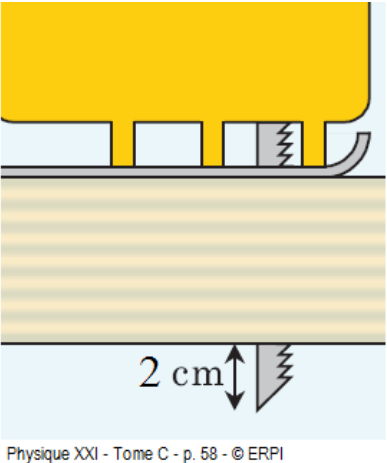
\includegraphics[width=1 \linewidth]{Figures/scie-sauteuse.png}
\end{minipage}

%\textbf{Mise en situation :} Après avoir survécu à votre session au Cégep, vous partez en vacances au village vacance lunaire. Alors que vous détendez vos muscles en apesanteur apparente dans le gymnase du complexe, un collègue vous défie de mesurer la masse d'un mystérieux haltère extraterrestre extrêmement dense. Vous n'avez évidemment pas pensé à apporter un pèse-personne dans vos bagages à main. Heureusement, votre trousse d'urgence contient un ressort parfait d'exercice physique !

\textbf{Problème :} Vous accrochez l'haltère au ressort dont la constante de rappel est $k = \BalleRaideur\text{ N/m}$. Vous étirez l'ensemble de $\BalleEtirement\text{ cm}$ depuis sa position d'équilibre, puis vous le relâchez sans vitesse initiale à $t = 0\text{ s}$. Vous observez que l'haltère repasse pour la toute première fois par sa position d'équilibre à l'instant $t = \BalleTempsPassage\text{ s}$.

\begin{enumerate}[label=\alph*)]
    \item Déterminez la période d'oscillation du système masse-ressort.
    \item Déterminez la masse de l'haltère mystérieux.
    \item Quelle est l'énergie mécanique totale emmagasinée dans le système ?
    \item Déterminez le module de la vitesse de l'haltère lorsqu'il atteint la position $x = \BallePosEval\text{ m}$.
\end{enumerate}
\vspace{15cm} \ \ \ 
\newpage

% Corde vs Tuyau
\subsection{(\rule{1cm}{0.4pt}/20 points)}

%
Le troisième mode d'une corde de guitare de longueur $L_c = \QtwoLc\text{ cm}$ fixée aux deux extrémités et de masse linéique $\QtwoMu\text{ kg/m}$ vibre à la même fréquence que le deuxième mode d'un tuyau ouvert-fermé de longueur $L = \QtwoLp\text{ cm}$. Le son voyage à $\QtwoVson\text{ m/s}$ ce jour-là.

\begin{enumerate}[label=\alph*)]
    \item Tracez l'allure générale du troisième mode de la corde et du deuxième mode du tuyau ouvert-fermé.
    \item Trouvez la tension de la corde.
    \item La corde de guitare vibre (toujours dans ce $3^\text{e}$ mode) et produit des ondes sonores. Quelles sont la fréquence et la longueur d'onde de ces ondes ?
\end{enumerate}
%
Une corde de guitare a une masse de $\QthreeMasse\text{ g}$ et une longueur de $\QthreeLcorde\text{ cm}$. Une flûte, considérée comme un tuyau ouvert aux deux bouts, a une longueur de $\QthreeLflute\text{ cm}$. Lorsque la corde de guitare vibre dans son deuxième mode, en même temps que la flûte vibre dans son mode fondamental, les deux instruments produisent des sons de même fréquence.

\begin{enumerate}[label=\alph*)]
    \item Tracez le schéma du mode de vibration de la corde et de la flûte. (4 pts)
    \item Déterminez la tension dans la corde de guitare. (12 pts)
    \item Quelle est la fréquence de la corde lorsqu'elle vibre dans son mode fondamental ? Quelle est alors la longueur d'onde de l'onde stationnaire sur la corde ? (schéma requis) (6 pts)
\end{enumerate}

Lors d'une répétition générale dans le département de musique, le deuxième mode de vibration d'une corde de contrebasse de longueur $L_c = \CordeLongueur\text{ cm}$ fixée aux deux extrémités et possédant une masse linéique de $\CordeMasseLin\text{ kg/m}$ résonne exactement à la même fréquence que le troisième mode d'un tuyau d'orgue fermé à une extrémité et ouvert à l'autre de longueur $L = \TuyauLongueur\text{ cm}$. La vitesse du son dans la pièce est évaluée à $\CordeVitesseSon\text{ m/s}$.

\begin{enumerate}[label=\alph*)]
    \item Tracez l'allure générale du deuxième mode de la corde et du troisième mode du tuyau ouvert-fermé.
    \item Calculez la tension appliquée sur la corde de contrebasse.
    \item La corde vibre (toujours dans son $2^\text{e}$ mode) et émet des ondes sonores dans l'air ambiant. Quelles sont la fréquence et la longueur d'onde de ces ondes sonores perçues dans la pièce ?
\end{enumerate}
% ------------------------------------------------------------------------------
% QUESTION A : Esquisse des modes de vibration
% ------------------------------------------------------------------------------
\subsubsection*{Question a) Allure générale des modes de vibration}

\begin{itemize}
    \item \textbf{Deuxième mode de la corde ($n = 2$, deux extrémités fixes) :} 
    La corde présente un nœud à chaque extrémité ainsi qu'un nœud central (soit 3 nœuds au total) et 2 ventres de vibration.
    
    \item \textbf{Troisième mode du tuyau fermé-ouvert ($n = 3$) :} 
    Pour un tuyau fermé à une extrémité et ouvert à l'autre, seuls les harmoniques impairs ($1, 3, 5, \dots$) existent. Le 3\textsuperscript{e} mode correspond au 5\textsuperscript{e} harmonique ($m = 5$). Il comporte un nœud à l'extrémité fermée et un ventre à l'extrémité ouverte, pour un total de 3 nœuds et 3 ventres.
\end{itemize}

\begin{center}
\begin{tikzpicture}[scale=0.9]
    % --- CORDE DE CONTREBASSE ---
    \begin{scope}[shift={(0,0)}]
        \node[anchor=east] at (-0.3,0) {\textbf{Corde ($n=2$) :}};
        % Extrémités fixes
        \fill[gray!50] (-0.2,-0.5) rectangle (0,0.5);
        \draw[thick] (0,-0.5) -- (0,0.5);
        \fill[gray!50] (6,-0.5) rectangle (6.2,0.5);
        \draw[thick] (6,-0.5) -- (6,0.5);
        % Axe
        \draw[dashed, gray] (0,0) -- (6,0);
        % Enveloppe du mode 2
        \draw[ultra thick, blue, domain=0:6, samples=100] plot (\x, {0.8*sin(2*180*\x/6)});
        \draw[ultra thick, blue, dashed, domain=0:6, samples=100] plot (\x, {-0.8*sin(2*180*\x/6)});
        % Nœuds et Ventres
        \foreach \x in {0, 3, 6} \fill[red] (\x,0) circle (2pt);
        \node[below, red, font=\scriptsize] at (0,-0.1) {N};
        \node[below, red, font=\scriptsize] at (3,-0.1) {N};
        \node[below, red, font=\scriptsize] at (6,-0.1) {N};
        \node[above, blue, font=\scriptsize] at (1.5,0.8) {V};
        \node[above, blue, font=\scriptsize] at (4.5,0.8) {V};
    \end{scope}

    % --- TUYAU ORGUE FERMÉ-OUVERT ---
    \begin{scope}[shift={(0,-2.5)}]
        \node[anchor=east] at (-0.3,0) {\textbf{Tuyau ($n=3$) :}};
        % Tuyau (Parois)
        \fill[gray!30] (0,-0.8) rectangle (0.2,0.8);
        \draw[thick] (0.2,0.8) -- (0,0.8) -- (0,-0.8) -- (0.2,-0.8);
        \draw[thick] (0,0.8) -- (6,0.8);
        \draw[thick] (0,-0.8) -- (6,-0.8);
        % Axe
        \draw[dashed, gray] (0,0) -- (6,0);
        % Ondes (5e harmonique : 2.5 quart d'onde sur L)
        \draw[ultra thick, orange!80!black, domain=0:6, samples=100] plot (\x, {0.7*sin(2.5*180*\x/6)});
        \draw[ultra thick, orange!80!black, dashed, domain=0:6, samples=100] plot (\x, {-0.7*sin(2.5*180*\x/6)});
        % Nœuds et Ventres
        \fill[red] (0,0) circle (2pt);
        \fill[red] (2.4,0) circle (2pt);
        \fill[red] (4.8,0) circle (2pt);
        \node[below, red, font=\scriptsize] at (0,-0.1) {N};
        \node[below, red, font=\scriptsize] at (2.4,-0.1) {N};
        \node[below, red, font=\scriptsize] at (4.8,-0.1) {N};
        \node[above, orange!80!black, font=\scriptsize] at (1.2,0.7) {V};
        \node[above, orange!80!black, font=\scriptsize] at (3.6,0.7) {V};
        \node[above, orange!80!black, font=\scriptsize] at (6,0.7) {V};
    \end{scope}
\end{tikzpicture}
\end{center}


% ------------------------------------------------------------------------------
% QUESTION B : Tension sur la corde
% ------------------------------------------------------------------------------
\subsubsection*{Question b) Calcul de la tension sur la corde de contrebasse}

\begin{enumerate}[label=\arabic*)]
    \item \textbf{Variables connues et recherchées :}
    \begin{itemize}[label= -]
        \item Longueur de la corde : $L_c = \qty{\CordeLongueur}{cm} = \qty{\fpeval{\CordeLongueur/100}}{m}$
        \item Masse linéique de la corde : $\mu = \qty{\CordeMasseLin}{kg/m}$
        \item Longueur du tuyau : $L_p = \qty{\TuyauLongueur}{cm} = \qty{\fpeval{\TuyauLongueur/100}}{m}$
        \item Vitesse du son dans l'air : $v_{\text{son}} = \qty{\CordeVitesseSon}{m/s}$
        \item Mode de la corde : $n_c = 2$ ($2^\text{e}$ harmonique)
        \item Mode du tuyau fermé-ouvert : $n_p = 3$ ($5^\text{e}$ harmonique)
        \item Variable recherchée : Tension dans la corde $T \text{ (N)}$
    \end{itemize}

    \item \textbf{Équations pertinentes :}
    \begin{itemize}[label= -]
        \item Fréquence du $3^\text{e}$ mode du tuyau fermé-ouvert ($5^\text{e}$ harmonique) :
        \[
        f_{p, 3} = \frac{5 v_{\text{son}}}{4 L_p}
        \]
        \item Fréquence du $2^\text{e}$ mode de la corde ($2^\text{e}$ harmonique) :
        \[
        f_{c, 2} = \frac{2 v_c}{2 L_c} = \frac{v_c}{L_c} \quad \text{avec} \quad v_c = \sqrt{\frac{T}{\mu}}
        \]
    \end{itemize}

    \item \textbf{Condition de résonance et isolation de $T$ :}
    Puisque les deux fréquences sont égales ($f_{c, 2} = f_{p, 3}$) :
    \[
    \frac{1}{L_c} \sqrt{\frac{T}{\mu}} = \frac{5 v_{\text{son}}}{4 L_p} \quad \implies \quad \sqrt{\frac{T}{\mu}} = \frac{5 L_c v_{\text{son}}}{4 L_p}
    \]
    En élevant au carré et en isolant la tension $T$ :
    \[
    T = \mu \cdot \left( \frac{5 L_c \cdot v_{\text{son}}}{4 L_p} \right)^2
    \]

    \item \textbf{Résolution numérique :}
    \[
    v_c = \frac{5 \cdot (\fpeval{\CordeLongueur/100}) \cdot \CordeVitesseSon}{4 \cdot (\fpeval{\TuyauLongueur/100})} = \qty{\fpeval{round((5 * \CordeLongueur * \CordeVitesseSon) / (4 * \TuyauLongueur), 2)}}{m/s}
    \]
    \[
    T = \CordeMasseLin \cdot \left( \fpeval{round((5 * \CordeLongueur * \CordeVitesseSon) / (4 * \TuyauLongueur), 4)} \right)^2 = \qty{\fpeval{round(\CordeMasseLin * ((5 * \CordeLongueur * \CordeVitesseSon) / (4 * \TuyauLongueur))^2, 2)}}{N}
    \]

    \item \textbf{Réponse :}
    La tension appliquée sur la corde de contrebasse est de \textbf{\qty{\fpeval{round(\CordeMasseLin * ((5 * \CordeLongueur * \CordeVitesseSon) / (4 * \TuyauLongueur))^2, 1)}}{N}}.
\end{enumerate}


% ------------------------------------------------------------------------------
% QUESTION C : Fréquence et longueur d'onde dans l'air
% ------------------------------------------------------------------------------
\subsubsection*{Question c) Fréquence et longueur d'onde des ondes sonores dans la pièce}

\begin{enumerate}[label=\arabic*)]
    \item \textbf{Variables connues et recherchées :}
    \begin{itemize}[label= -]
        \item Vitesse du son dans la pièce : $v_{\text{son}} = \qty{\CordeVitesseSon}{m/s}$
        \item Longueur du tuyau : $L_p = \qty{\fpeval{\TuyauLongueur/100}}{m}$
        \item Variables recherchées : Fréquence $f_{\text{son}} \text{ (Hz)}$ et longueur d'onde $\lambda_{\text{son}} \text{ (m)}$
    \end{itemize}

    \item \textbf{Équations pertinentes :}
    Lorsqu'une corde vibre, elle impose sa fréquence de vibration à l'air ambiant. Ainsi, la fréquence du son perçu est égale à la fréquence de vibration de la corde (et du tuyau) :
    \[
    f_{\text{son}} = f_{c, 2} = f_{p, 3} = \frac{5 v_{\text{son}}}{4 L_p}
    \]
    La longueur d'onde de ce son dans l'air dépend de la vitesse du son dans la pièce :
    \[
    \lambda_{\text{son}} = \frac{v_{\text{son}}}{f_{\text{son}}} = \frac{4 L_p}{5}
    \]

    \item \textbf{Résolution numérique :}
    \begin{itemize}[label= -]
        \item \textbf{Fréquence du son :}
        \[
        f_{\text{son}} = \frac{5 \cdot \CordeVitesseSon}{4 \cdot (\fpeval{\TuyauLongueur/100})} = \qty{\fpeval{round((5 * \CordeVitesseSon) / (4 * (\TuyauLongueur / 100)), 2)}}{Hz}
        \]
        \item \textbf{Longueur d'onde du son :}
        \[
        \lambda_{\text{son}} = \frac{4 L_p}{5} = \frac{4 \cdot (\fpeval{\TuyauLongueur/100})}{5} = \qty{\fpeval{round((4 * (\TuyauLongueur / 100)) / 5, 4)}}{m}
        \]
    \end{itemize}

    \item \textbf{Réponse :}
    Dans l'air ambiant de la pièce, l'onde sonore perçue a une fréquence de \textbf{\qty{\fpeval{round((5 * \CordeVitesseSon) / (4 * (\TuyauLongueur / 100)), 1)}}{Hz}} et une longueur d'onde de \textbf{\qty{\fpeval{round((4 * (\TuyauLongueur / 100)) / 5, 3)}}{m}} (soit \textbf{\qty{\fpeval{round(((4 * (\TuyauLongueur / 100)) / 5) * 100, 1)}}{cm}}).
\end{enumerate}

\newpage

% Puissance
\subsection{(\rule{1cm}{0.4pt}/20 points)}

\textbf{Mise en situation :} Vous assistez à un match de football du Noir et Or au terrain du Cégep. Alors que l'équipe locale réussit un touché spectaculaire en fin de partie, la sirène de but géante des partisans retentit avec éclat au bord du terrain pour célébrer la première victoire depuis plusieurs années.

\textbf{Questions :} Selon la fiche technique du matériel des partisans du Noir et Or, la puissance sonore émise à la source par cette sirène de but est de $\PneuPuissance\text{ W}$. Si vous mesurez un niveau d'intensité sonore de $\PneuNiveaudB\text{ dB}$ à l'endroit précis où vous êtes assis dans les gradins...

\begin{enumerate}[label=\alph*)]
    \item À quelle distance de la sirène de but vous trouvez-vous ?
    \item Quelle puissance acoustique exacte votre tympan absorbe-t-il si l'on modélise votre conduit auditif par un détecteur circulaire plat de rayon $\OreilleRayon\text{ m}$ ?
\end{enumerate}

Pour en ajouter une couche et faire vibrer la foule, le DJ du stade monte le son des haut-parleurs et fait jouer l'hymne de victoire du Noir et Or. Durant une pause entre deux coups de sirène (lorsque la sirène est silencieuse), vous mesurez le niveau sonore de la musique seule à $\MusiqueNiveaudB\text{ dB}$.

\begin{enumerate}[label= c)]
    \item Quel est le niveau d'intensité sonore total ressenti (en dB) lorsque la sirène de but retentit à nouveau pendant que la musique joue simultanément dans les haut-parleurs ?
\end{enumerate}

\subsubsection*{Question a) Distance par rapport à la sirène de but}

\begin{enumerate}[label=\arabic*)]
    \item \textbf{Variables connues et recherchées :}
    \begin{itemize}[label= -]
        \item Puissance de la source : $P = \qty{\PneuPuissance}{W}$
        \item Niveau d'intensité sonore : $\beta_{\text{sirène}} = \qty{\PneuNiveaudB}{dB}$
        \item Intensité du seuil d'audibilité : $I_0 = 10^{-12} \text{ W/m}^2$
        \item Variable recherchée : Distance $r \text{ (m)}$
    \end{itemize}

    \item \textbf{Équations pertinentes :}
    \[
    \beta = 10 \log_{10}\left(\frac{I}{I_0}\right) \quad \implies \quad I = I_0 \cdot 10^{\frac{\beta}{10}}
    \]
    \[
    I = \frac{P}{4\pi r^2} \quad \text{(modèle d'onde sphérique)}
    \]

    \item \textbf{Isolation de la variable recherchée :}
    \[
    \frac{P}{4\pi r^2} = I_0 \cdot 10^{\frac{\beta}{10}} \quad \implies \quad r^2 = \frac{P}{4\pi \cdot I_0 \cdot 10^{\frac{\beta}{10}}} \quad \implies \quad r = \sqrt{\frac{P}{4\pi \cdot I_0 \cdot 10^{\frac{\beta}{10}}}}
    \]

    \item \textbf{Résolution numérique :}
    \[
    I_{\text{sirène}} = 10^{-12} \cdot 10^{\frac{\PneuNiveaudB}{10}} = \num[scientific-notation=true, round-mode=figures, round-precision=3]{\fpeval{10^(-12) * 10^(\PneuNiveaudB / 10)}} \text{ W/m}^2
    \]
    \[
    r = \sqrt{\frac{\PneuPuissance}{4\pi \cdot 10^{-12} \cdot 10^{\frac{\PneuNiveaudB}{10}}}} = \qty{\fpeval{round(sqrt(\PneuPuissance / (4 * pi * 10^(-12) * 10^(\PneuNiveaudB / 10))), 2)}}{m}
    \]

    \item \textbf{Réponse :}
    Vous vous trouvez à une distance d'environ \textbf{\qty{\fpeval{round(sqrt(\PneuPuissance / (4 * pi * 10^(-12) * 10^(\PneuNiveaudB / 10))), 2)}}{m}} de la sirène de but.
\end{enumerate}


% ------------------------------------------------------------------------------
% QUESTION B
% ------------------------------------------------------------------------------
\subsubsection*{Question b) Puissance acoustique absorbée par le tympan}

\begin{enumerate}[label=\arabic*)]
    \item \textbf{Variables connues et recherchées :}
    \begin{itemize}[label= -]
        \item Rayon du conduit auditif : $R = \qty{\OreilleRayon}{m}$
        \item Intensité sonore locale : $I_{\text{sirène}} = \num[scientific-notation=true, round-mode=figures, round-precision=3]{\fpeval{10^(-12) * 10^(\PneuNiveaudB / 10)}} \text{ W/m}^2$
        \item Variable recherchée : Puissance absorbée $P_{\text{tympan}} \text{ (W)}$
    \end{itemize}

    \item \textbf{Équations pertinentes :}
    \[
    A = \pi R^2 \quad \text{(surface circulaire)}
    \]
    \[
    P_{\text{tympan}} = I_{\text{sirène}} \cdot A
    \]

    \item \textbf{Isolation de la variable recherchée :}
    \[
    P_{\text{tympan}} = \left( I_0 \cdot 10^{\frac{\beta}{10}} \right) \cdot \pi R^2
    \]

    \item \textbf{Résolution numérique :}
    \[
    A = \pi \cdot (\OreilleRayon)^2 = \num[scientific-notation=true, round-mode=figures, round-precision=3]{\fpeval{pi * (\OreilleRayon)^2}} \text{ m}^2
    \]
    \[
    P_{\text{tympan}} = \left(10^{-12} \cdot 10^{\frac{\PneuNiveaudB}{10}}\right) \cdot \pi (\OreilleRayon)^2 = \qty[scientific-notation=true, round-mode=figures, round-precision=3]{\fpeval{(10^(-12) * 10^(\PneuNiveaudB / 10)) * pi * (\OreilleRayon)^2}}{W}
    \]

    \item \textbf{Réponse :}
    La puissance acoustique exacte absorbée par le tympan est de \textbf{\qty[scientific-notation=true, round-mode=figures, round-precision=3]{\fpeval{(10^(-12) * 10^(\PneuNiveaudB / 10)) * pi * (\OreilleRayon)^2}}{W}} (soit environ \qty{\fpeval{round((10^(-12) * 10^(\PneuNiveaudB / 10)) * pi * (\OreilleRayon)^2 * 10^6, 2)}}{\micro\watt}).
\end{enumerate}


% ------------------------------------------------------------------------------
% QUESTION C
% ------------------------------------------------------------------------------
\subsubsection*{Question c) Niveau d'intensité sonore total (Superposition)}

\begin{enumerate}[label=\arabic*)]
    \item \textbf{Variables connues et recherchées :}
    \begin{itemize}[label=-]
        \item Niveau sonore de la sirène : $\beta_{\text{sirène}} = \qty{\PneuNiveaudB}{dB}$
        \item Niveau sonore de la musique : $\beta_{\text{musique}} = \qty{\MusiqueNiveaudB}{dB}$
        \item Intensité de référence : $I_0 = 10^{-12} \text{ W/m}^2$
        \item Variable recherchée : Niveau sonore total $\beta_{\text{tot}} \text{ (dB)}$
    \end{itemize}

    \item \textbf{Équations pertinentes :}
    \[
    I_{\text{tot}} = I_{\text{sirène}} + I_{\text{musique}} = I_0 \cdot 10^{\frac{\beta_{\text{sirène}}}{10}} + I_0 \cdot 10^{\frac{\beta_{\text{musique}}}{10}}
    \]
    \[
    \beta_{\text{tot}} = 10 \log_{10}\left(\frac{I_{\text{tot}}}{I_0}\right)
    \]

    \item \textbf{Isolation de la variable recherchée :}
    \[
    \beta_{\text{tot}} = 10 \log_{10}\left(\frac{I_0 \left(10^{\frac{\beta_{\text{sirène}}}{10}} + 10^{\frac{\beta_{\text{musique}}}{10}}\right)}{I_0}\right) = 10 \log_{10}\left(10^{\frac{\beta_{\text{sirène}}}{10}} + 10^{\frac{\beta_{\text{musique}}}{10}}\right)
    \]

    \item \textbf{Résolution numérique :}
    \[
    I_{\text{musique}} = 10^{-12} \cdot 10^{\frac{\MusiqueNiveaudB}{10}} = \num[scientific-notation=true, round-mode=figures, round-precision=3]{\fpeval{10^(-12) * 10^(\MusiqueNiveaudB / 10)}} \text{ W/m}^2
    \]
    \[
    I_{\text{tot}} = \num[scientific-notation=true, round-mode=figures, round-precision=3]{\fpeval{10^(-12) * (10^(\PneuNiveaudB / 10) + 10^(\MusiqueNiveaudB / 10))}} \text{ W/m}^2
    \]
    \[
    \beta_{\text{tot}} = 10 \log_{10}\left(10^{\frac{\PneuNiveaudB}{10}} + 10^{\frac{\MusiqueNiveaudB}{10}}\right) = \qty{\fpeval{round(10 * (ln(10^(\PneuNiveaudB / 10) + 10^(\MusiqueNiveaudB / 10)) / ln(10)), 2)}}{dB}
    \]

    \item \textbf{Réponse :}
    Le niveau d'intensité sonore total ressenti lorsque la sirène retentit en même temps que la musique est de \textbf{\qty{\fpeval{round(10 * (ln(10^(\PneuNiveaudB / 10) + 10^(\MusiqueNiveaudB / 10)) / ln(10)), 2)}}{dB}}.
\end{enumerate}

%
\textbf{Mise en situation :} Vous apercevez votre enseignant en train de jouer avec son animal de compagnie, Vincent le vélociraptor vorace, sur le terrain de football du cégep. Il lui lance son ballon de basketball préféré que Vincent va chercher en courant avant de le ramener à son maître qui le relance ensuite. Puis, tout à coup, le drame se produit : le ballon éclate.

\textbf{Questions :} Votre cours à option sur les dinosaures abordait justement la notion que la puissance sonore à la source du son produit par un vélociraptor enragé suite à la perte de son ballon était de $\QthreeP\text{ W}$. Si vous entendez un son de $\QthreeBeta\text{ dB}$, à l'endroit où vous vous trouvez...

\begin{enumerate}[label=\alph*)]
    \item À quelle distance vous trouvez-vous du dinosaure ?
    \item Quelle puissance votre oreille reçoit-elle si on l'assimile à un détecteur circulaire (plat) de rayon $\QthreeR\text{ m}$ ?
\end{enumerate}

Votre enseignant essaye de calmer les cris de son dinosaure en faisant jouer la chanson « Everybody Hertz » sur son téléphone cellulaire. Entre les cris du dinosaure (donc alors qu'il reprend son souffle et n'émet pas de son), vous entendez le niveau sonore de la musique à $\QthreeMusique\text{ dB}$.

\begin{enumerate}[label= c)]
    \item Quel est le niveau d'intensité sonore totale en dB lorsque vous entendez à la fois la musique et les cris du dinosaure ?
\end{enumerate}
%
Vous êtes dans un restaurant assez bruyant, où le niveau sonore est de $\QfourNiveau\text{ dB}$. Votre compagne de repas est assise devant vous, à une distance de $\QfourDist\text{ cm}$.

\begin{enumerate}[label=\alph*)]
    \item Quelle puissance sonore devrez-vous générer pour qu'elle vous entende avec une intensité sonore deux fois plus forte que celle du bruit ambiant ?
    \item Quel sera alors le niveau sonore perçu par votre compagne, en dB, en tenant compte du son de votre voix et du bruit ambiant ?
\end{enumerate}
\
\newpage

% Effet doppler
\subsection{(\rule{1cm}{0.4pt}/20 points)}

%
Albert et Béatrice ont commencé des leçons de saxophone. Les deux se déplacent vers vous, en jouant la même note, de fréquence $\QtwoFreq\text{ Hz}$. Albert marche à une vitesse de $\QtwoValb\text{ m/s}$, Béatrice à une vitesse de $\QtwoVbea\text{ m/s}$, tandis que vous marchez à $\QtwoVvous\text{ m/s}$ (voir le schéma pour la direction de ces vitesses). Quelle est la fréquence des battements que vous entendrez ?

\textit{(Tracez un schéma définissant clairement vos variables, justifiez vos choix de signes dans les équations, et expliquez pourquoi il y a un battement).}

\vspace{0.8cm}
\begin{center}
\begin{tikzpicture}[scale=1.1]
    % Albert
    \draw[thick, ->] (0,0) -- (1.2,0) node[midway, above] {$\QtwoValb\text{ m/s}$};
    \node at (0,-0.4) {\textbf{ALBERT}};
    
    % Vous
    \draw[thick, ->] (3.5,0) -- (4.7,0) node[midway, above] {$\QtwoVvous\text{ m/s}$};
    \node at (3.5,-0.4) {\textbf{VOUS}};
    
    % Béatrice
    \draw[thick, <-] (7,0) -- (8.2,0);
    \node at (7.6,0.3) {$\QtwoVbea\text{ m/s}$};
    \node at (7.6,-0.4) {\textbf{BÉATRICE}};
\end{tikzpicture}
\end{center}
\vspace{0.8cm}
%
Un chat poursuit un vélociraptor qui lui a volé son herbe à chat. Le vélociraptor terrorisé court à une vitesse de $\QfourVr\text{ m/s}$ (selon National Geographic), poursuivi par le chat qui court à une vitesse de $\QfourVc\text{ m/s}$. Durant la poursuite, le chat émet un miaulement de fréquence $\QfourFreq\text{ Hz}$. La vitesse du son ce jour-là est de $\QfourVson\text{ m/s}$.

\begin{enumerate}[label=\alph*)]
    \item Quelle est la fréquence de l'écho perçu par le chat (suite à la réflexion du miaulement sur le vélociraptor qu'il poursuit) ? Exceptionnellement, écrivez votre réponse avec quatre chiffres significatifs.
    \item Le chat entend une variation de l'intensité sonore entendue (l'intensité varie entre forte et faible). Quel est le nom de ce phénomène et avec quelle fréquence les moments de faible intensité se répètent-t-ils ?
\end{enumerate}

\vspace{0.4cm}

Dans un couloir du cégep, un faucon téméraire installé sur une trottinette électrique fonce à une vitesse de $\FauconVitesse\text{ m/s}$ en direction d'un robot-aspirateur sans défense qui tente d'échapper à l'impact en roulant dans la même direction à une vitesse de $\CibleVitesse\text{ m/s}$. Tout en fonçant, le faucon émet un huissement strident de fréquence $\OiseauFreq\text{ Hz}$. La vitesse du son dans le couloir est de $\DopplerVson\text{ m/s}$.

Un étudiant immobile se tient au centre du couloir, exactement entre le faucon et le robot-aspirateur.
    \begin{enumerate}[label=\alph*)]
        \item Quelle est la fréquence du son direct émis par le faucon et perçu par l'étudiant ?
        \item Quelle est la fréquence de l'écho provenant du robot-aspirateur et perçue par l'étudiant ?
        \item Quel est le nom du phénomène acoustique résultant de la réception simultanée de ces deux sons par l'étudiant, et quelle est la fréquence à laquelle ces moments de faible/forte intensité sonore se répètent ?
    \end{enumerate}

\vspace{0.4cm}
\begin{center}
\begin{tikzpicture}[scale=0.95, >=Stealth]
    % Sol du couloir
    \draw[thick] (-0.5,0) -- (11.0,0);
    \fill[gray!20] (-0.5,-0.2) rectangle (11.0,0);


    % Faucon sur trottinette (à gauche)
    \draw[thick, fill=gray!80] (0.5,0.2) circle (0.18);
    \draw[thick, fill=gray!80] (1.9,0.2) circle (0.18);
    \draw[ultra thick, blue!80!black] (0.5,0.2) -- (1.9,0.2);
    \draw[ultra thick, blue!80!black] (1.9,0.2) -- (1.9,1.5) -- (1.6,1.5);
    
    \draw[fill=orange!30, thick] (1.0,1.4) ellipse (0.45 and 0.3);
    \node[font=\small\bfseries] at (1.0,1.4) {Faucon};
    
    \draw[ultra thick, ->, blue!80!black] (1.0,2.1) -- (2.3,2.1) 
        node[midway, above, font=\small] {$v_f = \qty{\FauconVitesse}{m/s}$};

    % Étudiant immobile (au centre)
    \draw[thick, fill=green!20] (5.2,0.8) circle (0.25);
    \draw[thick] (5.2,0.55) -- (5.2,0.15);
    \draw[thick] (5.2,0.15) -- (5.0,0);
    \draw[thick] (5.2,0.15) -- (5.4,0);
    \draw[thick] (4.9,0.4) -- (5.5,0.4);
    \node[font=\small\bfseries, above] at (5.2,1.1) {Étudiant ($v_{\text{obs}}=0$)};

    % Robot-aspirateur (à droite)
    \draw[thick, fill=red!20] (8.2,0) arc (180:0:0.8 and 0.5) -- cycle;
    \draw[thick, fill=black] (8.5,0.1) circle (0.08);
    \draw[thick, fill=black] (9.5,0.1) circle (0.08);
    \node[font=\small\bfseries] at (9.0,0.25) {Robot};

    \draw[ultra thick, ->, red!80!black] (9.0,1.0) -- (10.2,1.0) 
        node[midway, above, font=\small] {$v_r = \qty{\CibleVitesse}{m/s}$};

    % Trajets des ondes sonores
    \draw[thick, cyan, ->] (1.9,1.2) -- (4.8,0.8) 
        node[midway, above, font=\scriptsize] {Direct ($f_{\text{dir}}$)};
    
    \draw[thick, cyan, dashed, ->] (1.9,1.5) .. controls (5.2,1.8) .. (8.2,0.8);

    \draw[thick, magenta, <-] (5.6,0.6) -- (8.2,0.4) 
        node[midway, below, font=\scriptsize] {Écho ($f_{\text{réfl}}$)};
\end{tikzpicture}
\end{center}

\vspace{0.3cm}

% ------------------------------------------------------------------------------
% QUESTION A
% ------------------------------------------------------------------------------
\subsection*{a) Fréquence du son direct perçu par l'étudiant}

\begin{enumerate}[label=\arabic*)]
    \item \textbf{Variables connues et recherchées :}
    \begin{itemize}[label=$\bullet$]
        \item Fréquence propre émise par le faucon : $f_0 = \qty{\OiseauFreq}{Hz}$
        \item Vitesse du faucon (source) : $v_{\text{source}} = v_f = \qty{\FauconVitesse}{m/s}$
        \item Vitesse de l'étudiant (observateur) : $v_{\text{obs}} = \qty{0}{m/s}$
        \item Vitesse du son dans le couloir : $v_s = \qty{\DopplerVson}{m/s}$
        \item Variable recherchée : Fréquence du son direct $f_{\text{dir}} \text{ (Hz)}$
    \end{itemize}

    \item \textbf{Équations pertinentes :}
    \[
    f' = f_0 \left( \frac{v_s \pm v_{\text{obs}}}{v_s \mp v_{\text{source}}} \right)
    \]

    \item \textbf{Isolation de la variable recherchée :}
    L'étudiant est immobile ($v_{\text{obs}} = 0$) et le faucon (source) s'approche de lui. La fréquence perçue doit donc être supérieure à la fréquence émise, ce qui impose un signe négatif $(-)$ au dénominateur :
    \[
    f_{\text{dir}} = f_0 \left( \frac{v_s}{v_s - v_f} \right)
    \]

    \item \textbf{Résolution numérique :}
    \[
    f_{\text{dir}} = \OiseauFreq \cdot \left( \frac{\DopplerVson}{\DopplerVson - \FauconVitesse} \right) = \qty{\fpeval{round(\OiseauFreq * (\DopplerVson / (\DopplerVson - \FauconVitesse)), 2)}}{Hz}
    \]

    \item \textbf{Réponse à la question :}
    La fréquence du son direct provenant du faucon et perçue par l'étudiant est de \textbf{\qty{\fpeval{round(\OiseauFreq * (\DopplerVson / (\DopplerVson - \FauconVitesse)), 2)}}{Hz}}.
\end{enumerate}



% ------------------------------------------------------------------------------
% QUESTION B
% ------------------------------------------------------------------------------
\subsection*{b) Fréquence de l'écho provenant du robot-aspirateur et perçue par l'étudiant}

\begin{enumerate}[label=\arabic*)]
    \item \textbf{Variables connues et recherchées :}
    \begin{itemize}[label=$\bullet$]
        \item Fréquence initiale du faucon : $f_0 = \qty{\OiseauFreq}{Hz}$
        \item Vitesse du faucon : $v_f = \qty{\FauconVitesse}{m/s}$
        \item Vitesse du robot-aspirateur : $v_r = \qty{\CibleVitesse}{m/s}$
        \item Vitesse du son : $v_s = \qty{\DopplerVson}{m/s}$
        \item Variable recherchée : Fréquence de l'écho perçu par l'étudiant $f_{\text{réfl}} \text{ (Hz)}$
    \end{itemize}

    \item \textbf{Équations pertinentes :}
    \begin{itemize}[label=-]
        \item \textit{Étape 1 (Faucon $\rightarrow$ Robot) :} Fréquence $f_r$ captée par le robot. Le faucon (source) s'approche $(-)$ et le robot (observateur) s'éloigne $(-)$ :
        \[
        f_r = f_0 \left( \frac{v_s - v_r}{v_s - v_f} \right)
        \]
        \item \textit{Étape 2 (Robot $\rightarrow$ Étudiant) :} Le robot réfléchit l'onde et agit comme une source émettant à la fréquence $f_r$ en s'éloignant $(+)$ de l'étudiant immobile ($v_{\text{obs}} = 0$) :
        \[
        f_{\text{réfl}} = f_r \left( \frac{v_s}{v_s + v_r} \right)
        \]
    \end{itemize}

    \item \textbf{Isolation de la variable recherchée :}
    En substituant $f_r$ dans la seconde équation, nous obtenons l'expression globale :
    \[
    f_{\text{réfl}} = f_0 \left( \frac{v_s - v_r}{v_s - v_f} \right) \left( \frac{v_s}{v_s + v_r} \right)
    \]

    \item \textbf{Résolution numérique :}
    \begin{itemize}[label=-]
        \item Fréquence reçue par le robot :
        \[
        f_r = \OiseauFreq \cdot \left( \frac{\DopplerVson - \CibleVitesse}{\DopplerVson - \FauconVitesse} \right) = \qty{\fpeval{round(\OiseauFreq * ((\DopplerVson - \CibleVitesse) / (\DopplerVson - \FauconVitesse)), 2)}}{Hz}
        \]
        \item Fréquence de l'écho réfléchie vers l'étudiant :
        \[
        f_{\text{réfl}} = \fpeval{round(\OiseauFreq * ((\DopplerVson - \CibleVitesse) / (\DopplerVson - \FauconVitesse)), 2)} \cdot \left( \frac{\DopplerVson}{\DopplerVson + \CibleVitesse} \right) = \qty{\fpeval{round(\OiseauFreq * ((\DopplerVson - \CibleVitesse) / (\DopplerVson - \FauconVitesse)) * (\DopplerVson / (\DopplerVson + \CibleVitesse)), 2)}}{Hz}
        \]
    \end{itemize}

    \item \textbf{Réponse à la question :}
    La fréquence de l'écho provenant du robot-aspirateur et perçue par l'étudiant est de \textbf{\qty{\fpeval{round(\OiseauFreq * ((\DopplerVson - \CibleVitesse) / (\DopplerVson - \FauconVitesse)) * (\DopplerVson / (\DopplerVson + \CibleVitesse)), 2)}}{Hz}}.
\end{enumerate}



% ------------------------------------------------------------------------------
% QUESTION C
% ------------------------------------------------------------------------------
\subsection*{c) Nom du phénomène acoustique et fréquence de répétition}

\begin{enumerate}[label=\arabic*)]
    \item \textbf{Variables connues et recherchées :}
    \begin{itemize}[label=$\bullet$]
        \item Fréquence du son direct : $f_{\text{dir}} = \qty{\fpeval{round(\OiseauFreq * (\DopplerVson / (\DopplerVson - \FauconVitesse)), 2)}}{Hz}$
        \item Fréquence du son réfléchi : $f_{\text{réfl}} = \qty{\fpeval{round(\OiseauFreq * ((\DopplerVson - \CibleVitesse) / (\DopplerVson - \FauconVitesse)) * (\DopplerVson / (\DopplerVson + \CibleVitesse)), 2)}}{Hz}$
        \item Variables recherchées : Nom du phénomène et fréquence des battements $f_{\text{batt}} \text{ (Hz)}$
    \end{itemize}

    \item \textbf{Équations pertinentes :}
    La superposition de deux ondes sonores de fréquences légèrement différentes engendre une variation périodique d'amplitude appelée \textbf{battements}.
    \[
    f_{\text{batt}} = |f_1 - f_2| = |f_{\text{dir}} - f_{\text{réfl}}|
    \]

    \item \textbf{Isolation de la variable recherchée :}
    \[
    f_{\text{batt}} = \left| f_0 \left( \frac{v_s}{v_s - v_f} \right) - f_0 \left( \frac{v_s - v_r}{v_s - v_f} \right) \left( \frac{v_s}{v_s + v_r} \right) \right|
    \]

    \item \textbf{Résolution numérique :}
    \[
    f_{\text{batt}} = \left| \fpeval{round(\OiseauFreq * (\DopplerVson / (\DopplerVson - \FauconVitesse)), 2)} - \fpeval{round(\OiseauFreq * ((\DopplerVson - \CibleVitesse) / (\DopplerVson - \FauconVitesse)) * (\DopplerVson / (\DopplerVson + \CibleVitesse)), 2)} \right| = \qty{\fpeval{round(abs((\OiseauFreq * (\DopplerVson / (\DopplerVson - \FauconVitesse))) - (\OiseauFreq * ((\DopplerVson - \CibleVitesse) / (\DopplerVson - \FauconVitesse)) * (\DopplerVson / (\DopplerVson + \CibleVitesse)))), 1)}}{Hz}
    \]

    \item \textbf{Réponse à la question :}
    Le phénomène acoustique s'appelle le \textbf{phénomène de battements}. Les moments de faible et de forte intensité sonore se répètent à une fréquence de \textbf{\qty{\fpeval{round(abs((\OiseauFreq * (\DopplerVson / (\DopplerVson - \FauconVitesse))) - (\OiseauFreq * ((\DopplerVson - \CibleVitesse) / (\DopplerVson - \FauconVitesse)) * (\DopplerVson / (\DopplerVson + \CibleVitesse)))), 1)}}{Hz}} (soit \fpeval{round(abs((\OiseauFreq * (\DopplerVson / (\DopplerVson - \FauconVitesse))) - (\OiseauFreq * ((\DopplerVson - \CibleVitesse) / (\DopplerVson - \FauconVitesse)) * (\DopplerVson / (\DopplerVson + \CibleVitesse)))), 1)} fois par seconde).
\end{enumerate}

\newpage

%%% Questions conceptuelles choisir 4-5 questions
\section{Questions conceptuelles (\rule{1cm}{0.4pt}/20 points)}

% Onde progressive

%\subsection{}
Une onde sinusoïdale progressive se propage sur une corde tendue (tension constante). La fonction d'onde est donnée par : $y = A \sin(k x - \omega t)$. Si on change la fréquence de la source, quels paramètres de la fonction d'onde seront modifiés ?

\begin{enumerate}[label=\Alph*)]
    \item $k$ seulement
    \item $\omega$ seulement
    \item $k$ et $\omega$
    \item $k$, $\omega$ et $A$
    \item $\omega$ et $A$
\end{enumerate}

\noindent\textbf{Justification :} \hrulefill \\[2.5ex]
\rule{\linewidth}{0.4pt} \\[2.5ex]
\rule{\linewidth}{0.4pt}
\vfill
\subsection{}
Deux cordes faites d'un même matériau sont attachées ensemble. La deuxième corde (celle de droite) a un diamètre plus grand. Une impulsion se déplace vers la droite dans la première corde, comme sur le schéma suivant :

\begin{center}
\begin{tikzpicture}[scale=0.9]
    \draw[thick] (-3,0) -- (-1.5,0) sin (-1,0.5) cos (-0.5,0) -- (0,0);
    \draw[line width=2.5pt] (0,0) -- (3,0);
    \draw[->, thick] (-1,0.7) -- (-0.5,0.7);
\end{tikzpicture}
\end{center}

Laquelle des images suivantes représente ce qui se passera après que l'impulsion ait atteint le point de jonction entre les deux cordes ?



\begin{center}
\begin{tikzpicture}[scale=0.85]
    % A
    \node at (-0.5, 3) {\textbf{A}};
    \draw[thick] (0,3) -- (0.5,3) sin (1,3.4) cos (1.5,3) -- (2.5,3);
    \draw[->] (1,3.6) -- (0.5,3.6);
    \draw[line width=2.5pt] (2.5,3) -- (3.5,3) sin (4,3.4) cos (4.5,3) -- (5.5,3);
    \draw[->] (4,3.6) -- (4.5,3.6);

    % C
    \node at (6.5, 3) {\textbf{C}};
    \draw[thick] (7,3) -- (7.5,3) sin (8,2.6) cos (8.5,3) -- (9.5,3);
    \draw[->] (8,2.4) -- (7.5,2.4);
    \draw[line width=2.5pt] (9.5,3) -- (10.5,3) sin (11,3.4) cos (11.5,3) -- (12.5,3);
    \draw[->] (11,3.6) -- (11.5,3.6);

    % B
    \node at (-0.5, 1) {\textbf{B}};
    \draw[thick] (0,1) -- (0.5,1) sin (1,1.4) cos (1.5,1) -- (2.5,1);
    \draw[->] (1,1.6) -- (0.5,1.6);
    \draw[line width=2.5pt] (2.5,1) -- (3.5,1) sin (4,0.6) cos (4.5,1) -- (5.5,1);
    \draw[->] (4,0.4) -- (4.5,0.4);

    % D
    \node at (6.5, 1) {\textbf{D}};
    \draw[thick] (7,1) -- (7.5,1) sin (8,0.6) cos (8.5,1) -- (9.5,1);
    \draw[->] (8,0.4) -- (7.5,0.4);
    \draw[line width=2.5pt] (9.5,1) -- (10.5,1) sin (11,0.6) cos (11.5,1) -- (12.5,1);
    \draw[->] (11,0.4) -- (11.5,0.4);

    % E
    \node at (3, -1) {\textbf{E}};
    \draw[thick] (3.5,-1) -- (6,-1);
    \draw[line width=2.5pt] (6,-1) -- (7,-1) sin (7.5,-0.6) cos (8,-1) -- (9,-1);
    \draw[->] (7.5,-0.4) -- (8,-0.4);
\end{tikzpicture}
\end{center}

\noindent\textbf{Justification :} \hrulefill \\[2.5ex]
\rule{\linewidth}{0.4pt} \\[2.5ex]
\rule{\linewidth}{0.4pt}
\vfill


% MHS

%\subsection{}
\begin{minipage}{0.7\textwidth}
 Un système masse-ressort oscillant à la verticale est fixé sur un moteur produisant une vibration. Lorsque le moteur est éteint et qu'on donne une poussée au bloc, il oscille avec une fréquence de $2\text{ Hz}$.

Après avoir immobilisé le bloc, on démarre le moteur. Laquelle des situations suivantes produira les oscillations de plus grande amplitude ?

\begin{enumerate}[label=\Alph*)]
    \item Si le moteur applique une force très intense
    \item Si le moteur applique une force faible mais constante
    \item Si le moteur vibre à une fréquence de $2\text{ Hz}$
    \item Si le moteur vibre à une fréquence très supérieure à $2\text{ Hz}$
    \item Si le moteur vibre à une fréquence très inférieure à $2\text{ Hz}$
\end{enumerate}
\end{minipage}%
\hfill
\begin{minipage}{0.25\textwidth}
\centering
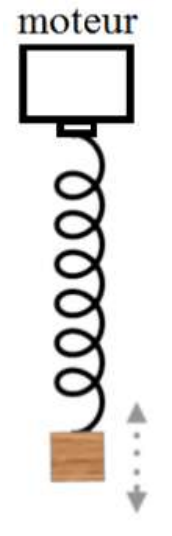
\includegraphics[width=0.45 \linewidth]{Figures/masse_ressort_general.png}
\end{minipage}

\vspace{0.3cm}

\noindent\textbf{Justification :} \hrulefill \\[2.5ex]
\rule{\linewidth}{0.4pt} \\[2.5ex]
\rule{\linewidth}{0.4pt}
\vfill
%\subsection{} On fait osciller un chariot contenant deux briques relié à deux ressorts. Si on enlève une des deux briques, la fréquence de l’oscillation sera-t-elle augmentée, diminuée ou inchangée ? Justifiez votre réponse.
\begin{center}
    \centering
    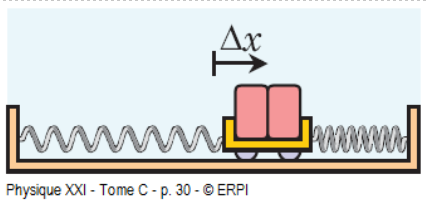
\includegraphics[width=0.45 \linewidth]{Figures/chariot_deux_briques.png}
\end{center}

\noindent\textbf{Réponse :} \hrulefill \\[2.5ex]
\rule{\linewidth}{0.4pt} \\[2.5ex]
\rule{\linewidth}{0.4pt}
\vfill
%\subsection{}
Au parc, Xavier se balance sur une balançoire, avec une période de $\mhsqCinqCPeriode$. Si son petit frère vient s’asseoir sur lui et qu’ils se balancent ensemble, la période de leur oscillation sera-t-elle plus grande, plus petite ou inchangée ? Justifiez votre réponse.

\noindent\textbf{Réponse :} \hrulefill \\[2.5ex]
\rule{\linewidth}{0.4pt} \\[2.5ex]
\rule{\linewidth}{0.4pt}
\vfill
%\subsection{}
Un système bloc-ressort effectue un mouvement harmonique simple à la fréquence $f$. Combien de fois par cycle est-ce que l’énergie cinétique de ce système sera égale à son énergie mécanique ?

\begin{enumerate}[label=\Alph*)]
    \item Une fois
    \item Deux fois
    \item Quatre fois
    \item Cela ne se produit jamais au cours d’un cycle.
\end{enumerate}

\noindent\textbf{Justification :} \hrulefill \\[2.5ex]
\rule{\linewidth}{0.4pt} \\[2.5ex]
\rule{\linewidth}{0.4pt}
\vfill
%\subsection{}
Une horloge à pendule utilise les oscillations harmoniques simples d’un pendule pour compter le passage des secondes. Supposons que vous avez une horloge à pendule de grande précision. Vous déménagez sur la Lune, où le champ gravitationnel est beaucoup moins intense, et vous emmenez votre horloge avec vous. Quelle modification devriez-vous faire pour que l’horloge marque le temps aussi bien sur la Lune que sur Terre ?

\begin{enumerate}[label=\Alph*)]
    \item Rien : l’horloge fonctionnera aussi bien sans aucune modification.
    \item Augmenter la masse du pendule.
    \item Diminuer la masse du pendule.
    \item Allonger la corde du pendule.
    \item Raccourcir la corde du pendule.
\end{enumerate}
\noindent\textbf{Justification :} \hrulefill \\[2.5ex]
\rule{\linewidth}{0.4pt} \\[2.5ex]
\rule{\linewidth}{0.4pt}
\vfill
%\subsection{}
Une masse fixée au bout d’un ressort oscille à la verticale. Si on donne une poussée à la masse de façon à augmenter l’amplitude de son oscillation, la période de l’oscillation sera-t-elle augmentée, diminuée ou inchangée ? (Justifiez votre réponse)

\noindent\textbf{Réponse :} \hrulefill \\[2.5ex]
\rule{\linewidth}{0.4pt} \\[2.5ex]
\rule{\linewidth}{0.4pt}
\vfill

\subsection{}
Lors d’un voyage à l’autre bout de la galaxie, un astronaute atterrit sur la planète WXZ4587-B, où la gravité est plus forte que sur Terre. Il a apporté avec lui, en souvenir de la Terre, un pendule et un système masse-ressort que lui avait donnés sa grand-mère. Sur Terre, les deux systèmes avaient la même fréquence d’oscillation. Sur WXZ4587-B, lequel des deux systèmes aura la plus basse fréquence ?

\begin{enumerate}[label=\Alph*)]
    \item Le pendule
    \item Le système masse-ressort
    \item La fréquence sera la même pour les deux
    \item Impossible de le savoir
\end{enumerate}
\noindent\textbf{Justification :} \hrulefill \\[2.5ex]
\rule{\linewidth}{0.4pt} \\[2.5ex]
\rule{\linewidth}{0.4pt}
\vfill
\subsection{}
Un trapéziste effectue un mouvement harmonique similaire à celui d’un pendule en se balançant de gauche à droite sur un fil. Lorsqu’il atteint sa hauteur maximum, sa collègue, qui était immobile sur une plateforme, s’accroche à ses mains et se laisse tomber avec lui. Quelle quantité ne sera pas modifiée par l’action de la deuxième trapéziste ?

\begin{enumerate}[label=\Alph*)]
    \item La vitesse des trapézistes à leur point le plus bas.
    \item La période d’oscillation des trapézistes.
    \item L’amplitude d’oscillation des trapézistes.
    \item Ces quantités seront toutes inchangées.
\end{enumerate}

\noindent\textbf{Justification :} \hrulefill \\[2.5ex]
\rule{\linewidth}{0.4pt} \\[2.5ex]
\rule{\linewidth}{0.4pt}
\vfill

% Onde stationnaire

\subsection{} 
Une onde sonore stationnaire (mode fondamental) est produite dans un tuyau ouvert aux deux bouts. Si la température de l'air dans le tuyau augmente, la fréquence sera ...

\begin{enumerate}[label=\Alph*)]
    \item augmentée
    \item diminuée
    \item inchangée
    \item impossible de le savoir
\end{enumerate}

\noindent\textbf{Justification :} \hrulefill \\[2.5ex]
\rule{\linewidth}{0.4pt} \\[2.5ex]
\rule{\linewidth}{0.4pt}
\vfill

% Doppler
\subsection{}
Un émetteur (E) d’une onde sonore et deux récepteurs (R1 et R2) voyagent à vitesse $v$, plus petite que la vitesse du son, dans les directions indiquées (R1 et E se déplacent vers la droite, R2 se déplace vers la gauche). Lequel des deux récepteurs recevra le son avec la plus grande fréquence ?
\begin{figure}[h]
    \centering
    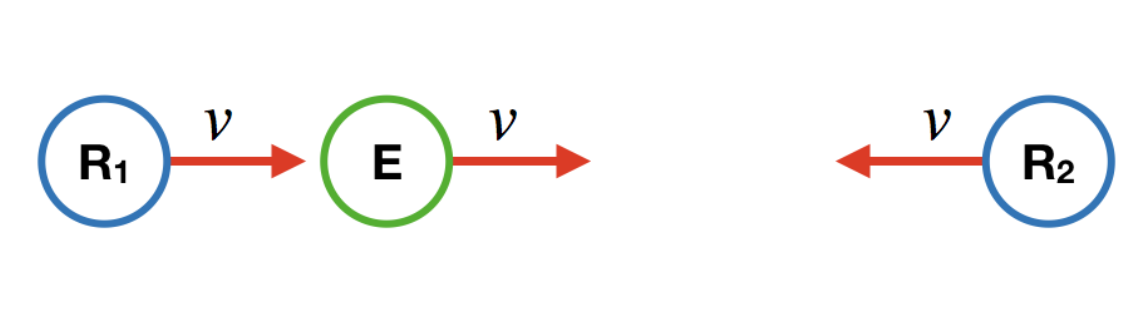
\includegraphics[width=0.9\linewidth]{Figures/1emetteur2recepteur.png}
\end{figure}
\begin{enumerate}[label=\Alph*)]
    \item Le récepteur R1.
    \item Le récepteur R2.
    \item Les deux récepteurs reçoivent un son avec une fréquence identique.
    \item Impossible de le savoir sans connaître la valeur de la vitesse $v$.
\end{enumerate}

\noindent\textbf{Justification :} \hrulefill \\[2.5ex]
\rule{\linewidth}{0.4pt} \\[2.5ex]
\rule{\linewidth}{0.4pt}
\vfill
%\subsection{}
Un camion de pompier roulant à $\doppDeuxCVitCamion$ dépasse une auto qui avance à $\doppDeuxCVitAuto$ dans la même direction. La vitesse de propagation de l’onde sonore émise par le camion de pompier sera :
\begin{enumerate}[label=\Alph*)]
    \item La même que la vitesse de propagation des ondes sonores du klaxon de l’auto.
    \item Deux fois plus grande que la vitesse de propagation des ondes sonores du klaxon de l’auto.
    \item Plus grande que la vitesse de propagation des ondes sonores du klaxon de l’auto, mais pas deux fois plus grande.
    \item Deux fois plus petite que la vitesse de propagation des ondes sonores du klaxon de l’auto.
    \item Plus petite que la vitesse de propagation des ondes sonores du klaxon de l’auto, mais pas deux fois plus petite.
\end{enumerate}

\noindent\textbf{Justification :} \hrulefill \\[2.5ex]
\rule{\linewidth}{0.4pt} \\[2.5ex]
\rule{\linewidth}{0.4pt}
\vfill

% Battements

% Onde sinusoidale

% Puissance
%\subsection{}
Plusieurs haut-parleurs identiques sont placés côte à côte à la même distance de l’observateur; ils produisent ensemble une intensité sonore de $\doppUnCIntensite \text{ dB}$. Si on n'en laisse fonctionner qu'un seul, quelle est l’intensité sonore produite ? Expliquez votre réponse.

\begin{enumerate}[label=\Alph*)]
    \item $25\text{ dB}$
    \item $27\text{ dB}$
    \item $30\text{ dB}$
    \item $33\text{ dB}$
\end{enumerate}

\noindent\textbf{Justification :} \hrulefill \\[2.5ex]
\rule{\linewidth}{0.4pt} \\[2.5ex]
\rule{\linewidth}{0.4pt}
\vfill


\hfill \textbf{Total : 100 points}

\end{document}